\begin{frame}[t]{C\'omo usar el software?}\vspace{0pt}
Dentro del Jupyter Notebook:
\begin{enumerate}
	\item  Ingresa a la pesta\~na ``datos" y selecciona el nombre del archivo de texto que contiene la matriz experimental que deseas analizar. Para guardar la matriz, ejecuta el siguiente bloque de c\'odigo.
	\begin{figure}
		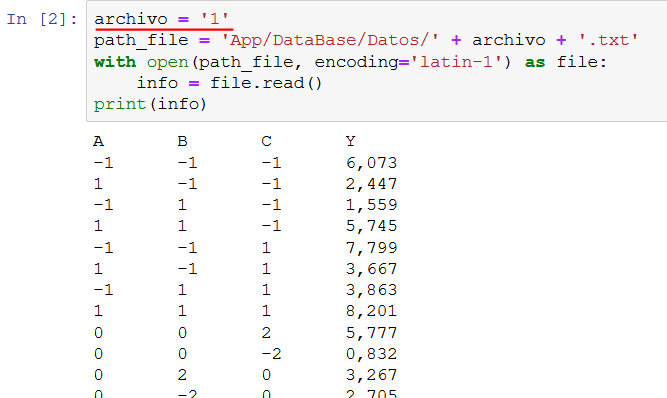
\includegraphics[scale=0.55]{Images/data.png}
	\end{figure}
	\item El orden de ejecuci\'on de los enlaces es: ``datos", ``modelo" y ``validaci\'on", respectivamente.
\end{enumerate}
\end{frame}